% Chapter 6

\chapter{Experiment A} % Main chapter title

\label{Chapter6} % For referencing the chapter elsewhere, use \ref{Chapter1}

%----------------------------------------------------------------------------------------

\begin{itquote}
Q: Why did the multithreaded chicken cross the road?
A: to To other side . get the
\flushright
\textsc{Jason Whittington}
\end{itquote}

\section{Idee}

Gegeben ist ein Vektorraum $V$ mit Wortvektoren $\vec{u}, \vec{v} \in V$ und $\vec{u},\vec{v}\in\mathbb{R}^d$.
Gesucht ist eine Funktion $\phi$, die ein Vektorenpaar in einen Relationsraum abbildet: $\phi: \mathbb{R}^d \to \mathbb{R}^e$, wobei
nicht zwangsläufig $d = e$.\\
In ihrer einfachsten Form bildet sie einfach die Differenz $\vec{d}$ der beiden Vektoren:
\begin{equation}
  \phi(\vec{u}, \vec{v}) = \vec{v} - \vec{u} = \vec{d}
\end{equation}

\section{Algorithmus}

Der Grundalgorithmus (siehe Fig. X) versucht nun, alle Kombinationen von Wortvektoren zu bilden und über diese
und den Differenzvektor zu bilden. Alle Kombinationen würde bei $n$ Vektoren in $n * n = n^2$ Vektoren resultieren.
Zwar ist $\phi(\vec{u}, \vec{v}) \neq \phi(\vec{v}, \vec{u})$, jedoch wäre die Berechnung beider Differenzvektoren redundant,
da sie lediglich Spiegelungen voneinander im Raum sind und so diesselbe Information enthalten. Die Berechnung
der Differenz in nur eine Richtung reduziert die Anzahl der Vektoren dadurch zu $\frac{n * (n-1)}{2}$.

\begin{figure}[h]
  \centering
  \begin{algorithm}[H]
    \KwData{Menge von Vektorpaaren $\mathcal{C}$}
    \For{$(\vec{u}, \vec{v}) \in \mathcal{C}$}{
      $\vec{d} = \vec{v} - \vec{u}$;
    }
  \end{algorithm}
  \caption[Einfacher Projektionsalgorithmus]{Einfacher Projektionsalgorithmus.}
\end{figure}

Gegeben einer Menge relevanter Kombinationen $\mathcal{C}$ mit Vektorpaaren gilt also:
\begin{equation}
  \forall (\vec{u}, \vec{v}) \in \mathcal{C}: (\vec{v}, \vec{u}) \notin \mathcal{C}
\end{equation}

Eine Modifikation des Algorithmus besteht daran, das Berechnen von $\vec{d}$ ab eine Bedingung zu knüpfen.
Gegeben sei eine Menge von Sätzen (ein Korpus) $\mathcal{K}$ mit $n$ Sätzen $s_i$ sodass $\mathcal{K} = \{s_i\}_{i=1}^{n}$ mit
$m$ Wörtern $w_{ij}$ pro Satz $s_i = \{w_{ij}\}_{j=1}^m$. Eine Kookkurrenz von zwei Begriffen (\emph{types}) $t_1$ und $t_2$
besteht demnach, falls im Korpus mindestens ein Satz existiert, in dem beide gleichermaßen vorkommen. Dazu können wir
eine Funktion $\Lambda$ definieren, die die Anzahl der Kookkurrenzen bestimmt:
\begin{equation}
  \Lambda(t_1, t_2) = |\{s_i | \exists w_{ij} = t_1 \land \exists w_{ij} = t_2 \land t_1\neq t_2\}_{i=1}^{n}|
\end{equation}
Eine mögliche Einschränkung besteht darin, in einem geänderten Algorithmus (siehe Fig. X) das Berechnen von $\vec{d}$ nur
dann zu erlauben, wenn die Anzahl der Kookkurrenzen der zu den Vektoren $\vec{v}(t_1), \vec{v}(t_2)$ gehörenden Begriffe $t_1, t_2$
einen bestimmten Schwellenwert $\gamma$ überschreitet, also $\Lambda(t_1, t_2) > \gamma$.

\begin{figure}[h]
  \centering
  \begin{algorithm}[H]
    \KwData{Menge von Vektorpaaren $\mathcal{C}$}
    \For{$(\vec{v}(t_1), \vec{v}(t_2)) \in \mathcal{C}$}{
      \If{$\Lambda(t_1, t_2) > \gamma$}{
        $\vec{d} = \vec{v}(t_2) - \vec{v}(t_1)$;
      }
    }
  \end{algorithm}
  \caption[Modifizierter Projektionsalgorithmus]{Modifizierter Projektionsalgorithmus, bei dem die zu den Vektoren gehörigen
  Begriffe über $\gamma$ Mal im Korpus im gleichen Satz aufgetreten sein müssen, damit $\vec{d}$ errechnet wird.}
\end{figure}


\section{Parallelisierter Algorithmus}

Doch selbst mit den erwähnten Einschränkungen skaliert dieser Algorithmus nur bedingt. Um dem entgegenzuwirken, soll nun
versucht werden, diesen mithilfe von \emph{Multithreading} zu parallelisieren. Bei dieser Technik beschäftigt ein Rechenprozess
mehrere Prozessstränge (\emph{Threads}), die miteinander kommunizieren und bei Bedarf synchronisiert werden können,
während sie Teile eines Problems lösen.\\
Ein beliebtes Muster, das Verhältis zwischen mehreren Threads zu definieren besteht im \emph{Master-Slave}-Muster.
Dabei fungiert ein Subprozess als Aufseher, der seine Arbeiterprozesse überwacht, sie mit Daten versorgt und in manchen
Fällen untereinander koordiniert.\\ \\

\begin{figure}[h]
  \centering
  \begin{algorithm}[H]
    \KwData{Menge von Vektorpaaren $\mathcal{C}$}
    \KwData{Menge von erledigten Vektorpaaren $\mathcal{C}'$ (Anfangs $\mathcal{C}' = \varnothing$)}
    \KwData{Menge von Threads $\mathcal{T}=\{th\}_i^n$}
    \BlankLine
    \textbf{Klasse} \textsc{MasterThread} \\
      data = ladeDaten();\\
      \For{$th \in \mathcal{T}$}{
        starteThread($th$, data);
      }
      \For{$th \in \mathcal{T}$}{
        beendeThread($th$);
      }

    \BlankLine
    \textbf{Klasse} \textsc{WorkerThread} \\
    \For{$(\vec{v}(t_1), \vec{v}(t_2)) \in \mathcal{C}$}{
      \If{$(\vec{v}(t_1), \vec{v}(t_2)) \notin \mathcal{C}'$}{
        \If{$\Lambda(t_1, t_2) > \gamma$}{
          $\vec{d} = \vec{v}(t_2) - \vec{v}(t_1)$;
        }
        $\mathcal{C}'$ = $\mathcal{C}' \cup (\vec{v}(t_1), \vec{v}(t_2))$;
      }
    }
  \end{algorithm}
  \caption[Parallelisierter Projektionsalgorithmus]{Parallelisierter Projektionsalgorithmus, bei dem die zu den Vektoren gehörigen
  Begriffe über $\gamma$ Mal im Korpus im gleichen Satz aufgetreten sein müssen, damit $\vec{d}$ errechnet wird. Ein Master-Thread
  verteilt zudem die Aufgaben an Worker-Threads, die diese Berechnungen übernehmen und erledigt Vektorpaare in einer Menge ablegen.}
\end{figure}

In diesem konkreten Fall ist der Master-Thread dafür verantwortlich, alle benötigten Daten in entsprechende Datenstrukturen
zu laden, sie den Worker-Threads bereitzustellen und letztere gemeinsam zu starten und zu beenden, sobald ein bestimmtes
Abschlusskriterium der Aufgabe erfüllt ist.
Zusätzlich wird eine Menge eingeführt, in die Paare von Vektoren hinzugefügt werden, sofern für sie von einem Thread
ein Differenzvektor ausgerechnet wurde. Damit nun keiner der Threads redundante Berechnungen durchführt, prüft er, ob sein
aktuelles Vektorpaar sich in dieser Menge befindet und schon abgehakt wurde\footnote{Damit dies möglichst schnell funktioniert,
wird das Vektorpaar durch eine Hashfunktion in einen Wert umgewandelt. Diese wird so gewählt,
sodass $h(\vec{v}(t_1), \vec{v}(t_2)) = h(\vec{v}(t_2), \vec{v}(t_1))$.}.\\

Als Grundlage der Daten wurde das Datenset Mark 0 [BESTES EINFÜGEN] gewählt, da es in den meisten der Evaluationsaufgaben
als bestes Abschnitt. Mit $\gamma = 100$ resultierte das Procedere in einem neuen Menge an Daten mit insgesamt
X Differenzvektoren [GENAUE ZAHL EINFÜGEN] mit einer Größe von X,X GB [GENAUE GRÖSSE EINFÜGEN].\\
Um den Gewinn durch Multithreading zu verdeutlichen, wurden darüber hinaus die Rechenzeiten gemessen (siehe Fig. X).
Gerechnet wurde auf eine Hardware mit 40 Prozessorkernen und [RESTLICHE SPECS EINFÜGEN].

\begin{figure}[h]
  \centering
  \begin{tabular}{r|cc}
    \textsc{Anzahl der Threads} & \textsc{Benötigte Zeit} (in $m$) & Beschleunigung (in \%) \\
    \hline
    1 & & - \\
    2 & & \\
    8 & & \\
    32 & & \\
    64 & & \\
    128 & & \\
  \end{tabular}
  \caption[Rechenzeiten für den Mappingschritt nach Anzahl von Threads]{Rechenzeiten für den Mappingschritt nach Anzahl von Threads auf
  einem System mit 40 Prozessorkernen und [RESTLICHE SPECS EINFÜGEN]. Die Beschleunigung wird im Vergleich zum Ausführen des Programms
  mit nur einem Thread gemessen.}
\end{figure}

\section{Clustering}

\emph{Clustering} bezeichnet eine Art von unüberwachten maschinellen Lernen,
die versucht, Elemente, die nach vorher definierten Maßgaben als ähnlich erachtet
werden sollen, zu gruppieren.\\
Die Literatur zu diesem Thema bietet dabei eine Fülle von Algorithmen mit verschiedenen
Grundannahmen, aus denen es zu wählen gilt. Für die Aufgaben in dieser Arbeit wurde
der DBSCAN-Algorithmus (\textbf{D}ensity-\textbf{B}ased \textbf{S}patial \textbf{C}lustering of
\textbf{A}pplications with \textbf{N}oise) gewählt, da er folgende Kriterien erfüllt:
\begin{itemize}
  \item DBSCAN erlaubt es, dass nicht alle Datenpunkte bei der
  Terminierung des Algorithmus einem Cluster zugeordnet sein müssen (\emph{Outlier detection})
  \item Die Anzahl der Cluster muss bei Beginn des Algorithmus nicht festgelegt werden.
  \item Cluster werden nicht nach der räumlichen Distanz zwischen den Punkten gebildet, sondern nach deren
  Dichte im Raum. Dies lässt auch nicht-sphärische Clusterformen zu.
\end{itemize}

Zur Erklärung von DBSCAN müssen zuerst einige Definitionen erstellt werden:
\begin{itemize}
  \item Ein Punkt $p$ in den Daten wird dann als
  Kernpunkt (\emph{core point}) bezeichnet, sofern mindesten $minPts$ Punkte innerhalb einem Radius $\epsilon$ vorhanden sind.\\
  Diese Punkte sind von $p$ \emph{direkt erreichbar}.
  \item Ein Punkt $q$ ist von $p$ erreichbar, sofern es einen Pfad $p_1, \ldots, p_n$ mit $p_1 = p$ und $p_n = q$ gibt, wobei
  jeder Punkt $p_{i+1}$ von einem Punkt $p_i$ direkt erreichbar ist.
  \item Alle Punkte, die nicht von einem anderen Punkt aus direkt erreichbar sind, sind Ausreißer (\emph{Outlier}).
  \item Zwei Punkte $p$ und $q$ sind \emph{direkt verbunden}, sofern es einen Punkt $o$ gibt,
  von dem aus beide Punkte direkt erreichbar sind.
  \item Cluster bestehen aus Punkten, die alle miteinander direkt verbunden sind.
\end{itemize}

\begin{figure}[h]
  \centering
  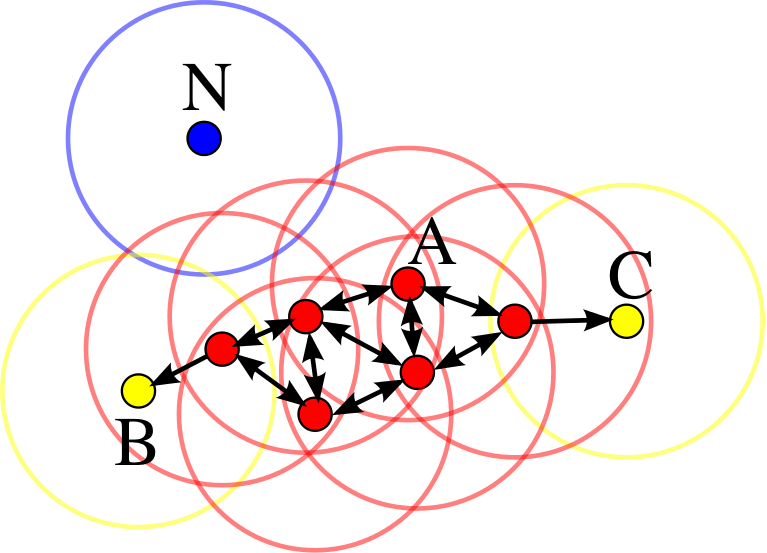
\includegraphics[width=0.6\textwidth]{../img/DBSCAN-Illustration.png}
  \caption[Darstellung der Funktionsweise von DBSCAN]{Darstellung der Funktionsweise von DBSCAN. Punkt A ist ein Kernpunkt, die
  Punkte B und C sind von A aus erreichbar. Punkt N ist nicht erreichbar und damit ein Ausreißer.\footnotemark}
\end{figure}
\footnotetext{Abbildung von
Chire - Eigenes Werk, CC BY-SA 3.0, \url{https://commons.wikimedia.org/w/index.php?curid=17045963} (zuletzt abgerufen am
25.04.16).}

Der Algorithmus ist von linearer Komplexität, sofern ihm eine geeignete Indexierung der Daten zugrunde gelegt wird, ansonsten
verhält sich die Komplexität quadratische zur Anzahl der Datenpunkte\footnote{Bei der
\verb|scikit-learn|-Implementation wird beispielsweise ein Nearest-Neighbour-Graph verwendet:
\url{http://scikit-learn.org/stable/modules/generated/sklearn.cluster.dbscan.html} (zuletzt abgerufen am 25.04.16)}.

\section{Ergebnisse}

\section{Zwischendiskussion}

Wie der letzte Abschnitt der gezeigt hat, entsprechen die Ergebnisse nicht den vorher gefassten Hoffnungen.
Im Folgenden soll ein Versuch unternommen zu erklären, welche Probleme zu diesen Resultaten geführt haben und welche
Implikationen diese besitzen.

\subsection{Daten}

Will man das Scheitern unmittelbar auf einen Faktor zurückführen, so liegen die zugrunde liegenden Daten am nächsten.
Es lassen sich im Bezug auf jene folgende Punkte feststellen:
\begin{itemize}
  \item \textbf{Menge}\\ Selbst mit dir Reduzierung der resultierenden Daten von $n^2$ auf $\frac{n*(n-1)}{2}$ ist die
  Datenmenge noch sehr groß, gerade wenn das anfänglich Wortvektorset auf einem großen Vokabular wie dem des Decow-Korpus aufbaut.
  Dies stellt hohe Anforderung an die Skalierbarkeit aller involvierter Algorithmen und fordert Einschränkungen auf verschiedener
  Ebene, wodurch mögliche spätere Entdeckung eventuell vorenthalten werden könnten.
  \item \textbf{Rauschen}\\ In den Enddaten ist der überwiegende Teil der Datenpunkte keiner sinnvollen Relation zuzuordnen.
  Dadurch verrauschen diese mögliche sinnvolle Relationscluster, die darin untergehen. Die resultierenden Cluster sind sehr
  schwammig, da sie sich schlecht vom Hintergrundrauschen abgrenzen. Dies ist beispielsweise durch den Wert des Silhouettenkoeffizienten
  \footnote{Der Silhoettekoeffizient $s_C$ beschreibt das durchschnittliche Verhältnis vom Abstand eines Punktes zu seinem Clusterzentrum gegnüber
  des nächsten Clusterzentrums. $-1 \leq s_C \leq 1$.}
  erkennbar, der bei den Experimenten immer kurz unter Null lag\footnote{Für ein gutes Clustering wird ein Wert von $s_C \geq 0,75$
  erwartet.}.
  \item \textbf{Ähnliche Distanzvektoren}\\
  Der beschriebene Ansatz wurde unter der Annahme verfolgt, dass für Wortpaare einer Relation $R=\{(h_j, t_j\}_{j=0}^m$
  folgendes gilt:
  \begin{equation}
    \vec{v}(t_0) - \vec{v}(h_0) \approx \vec{v}(t_1) - \vec{v}(h_1) \approx \ldots \approx \vec{v}(t_m) - \vec{v}(h_m)
  \end{equation}
  Anders ausgedrückt wurde aufgrund vorheriger Arbeiten die Hypothese aufgestellt, dass sich die Distanzvektoren von
  Wortpaaren derselben Relation ähneln. Durch die Ergebnisse wurde diese Hypothese nicht widerlegt (im Gegenteil scheinen
  andere Arbeiten wie (\cite{bordes2013translating}) oder (\cite{lin2015learning}) diese Annahmen zu bestätigen), jedoch
  gilt diese Eigenschaft nicht \textbf{exklusiv} für diese Untermenge an Vektorenpaaren.\\
  Nehmen wir beispielsweise im ursprünglichen Vektorraum mit Wortvektoren das folgende Szenario an: Wir finden dort
  zwei Cluster $C_1$ und $C_2$ vor. Die zu den Vektoren zugehörigen Cluster weisen eine semantische Ähnlichkeit auf
  und liegen deshalb nahe beieinander, z.B. Vornamen wie \emph{Julia} und \emph{Hans} in $C_1$ und Städte wie
  \emph{Barcelona} und \emph{Paris} in $C_2$. Daraus ergibt sich Folgendes:
  \begin{equation}
    \begin{split}
      \vec{v}(Julia) \approx \vec{v}(Hans) \land \vec{v}(Barcelona) \approx \vec{v}(Paris) \implies \\
      \vec{v}(Julia) - \vec{v}(Barcelona) \approx \vec{v}(Hans) - \vec{v}(Paris)
    \end{split}
  \end{equation}
  Anders ausgedrückt: Auch wenn sich semantische Information in den Wortvektoren dadurch manifestiert, dass ähnliche
  Ausdrücke in ihren Clustern nahe beinander liegen, können Distanzvektoren aus Wortenpaaren der gleichen Cluster ähnlich sein,
  ohne semantisch in irgendeinem Zusammenhang zu stehen. Dies führt schlussendlich dazu, dass die wenigen Cluster, die
  im Relationsraum gefunden werden, zwar aus Wortpaaren mit ähnlichem Differenzvektor stehen, jedoch keine ``sinnvolle''
  Relation bilden, was sicht mit dem in 6.1 eingeführtern Parameter $\gamma$ zwar verringern, allerdings nicht gänzlich
  verhindern lässt. Das Ziel, neue und legitime Relationen zu finden, wird durch diesen Trugschluss ad absurdum geführt.

\end{itemize}

\subsection{Ansatz}

Das Fehlschlagen des Vorgehens kann auch auf einer theoretischen Ebene festgestellt werden: Das Ziel bestand darin, Wissen
über Relationen zwischen Wortpaaren zu extrahieren. Um dieses Wissen gewissermaßen ``freilegen'', muss es aber auf eine
Art und Weise innerhalb der Daten ``kodiert'' sein, wenn auch versteckt (so wie die semantische Ähnlichkeit zwischen Wörtern
durch die räumliche Nähe ihrer Vektoren und deren Dimension kodiert ist).\\
Wie beim Aufzeigen des Trugschlusses am Ende des vorherigen Abschnitts gezeigt wurde, sind semantische Relationen nicht eindeutig
innerhalb der Daten aufzuzeigen bzw. nur dann, wenn bereits vorher bruchstückhaftes Wissen darüber vorliegt. Ohne
dieses Vorwissen sind richtige von nur scheinbaren Relationen nicht zu trennen.
